\subsection{ Filter Attenuation }
A simple low pass filter can be formed from a resistor and a capacitor in series.

\begin{figure}[h]
  \centering
\begin{circuitikz}
\draw (0,0) to [short,*-,l=$V_{in}$] (1,0)
  to [european resistor, l=$R$] (3,0)
  to [C,l=$C$] (3,-2)
  to (3,-2) node[ground]{};
\draw (3,0) to [short,-*,l=$V_{out}$] (5,0);
\end{circuitikz}
\caption{Circuit diagram for a RC low pass filter.} \label{fig:RC_low_pass_circuit}
\end{figure}
We can see from figure \ref{fig:RC_low_pass_circuit}, that the output voltage is
the same as the voltage across the capacitor. So we have
\begin{align}
V_{in} &= V_{R} + V_{C} \nonumber \\
       &= IR + V_{out}
\end{align}
Using the fact that the current through the RC section of the circuit is given
by
\begin{equation}
  I = \frac{V_{in}}{R - i X_C}
\end{equation}
Leading to the output voltage being
\begin{align}
V_{out} &= V_{in} - IR \nonumber \\
&= V_{in} - \frac{V_{in}R}{R - i X_C} \nonumber  \\
&= V_{in}\left[ 1 - \frac{V_{in}R}{R - i X_C} \right]
\end{align}
which leads to a ratio of the output voltage to the input voltage of
\begin{align}
\frac{V_{out}}{V_{in}} &= 1 - \frac{R}{R - i X_C} \nonumber \\
&= \frac{-i X_C}{R - i X_C} \nonumber \\
&= \frac{-i X_C(R+iX_C)}{R^2+{X_C}^2} \label{eq:RC_volt_ratio}
\end{align}
Now if we let
\begin{equation}
u = \frac{R}{X_c} = \omega R C \label{eq:RC_u}
\end{equation}
we can see that $R=uX_C$, and putting this in equation \ref{eq:RC_volt_ratio} leads to
\begin{align}
\frac{V_{out}}{V_{in}} &= \frac{-i {X_C}^2(u+i)}{u^2{X_C}^2+{X_C}^2} \\
&= \frac{1-iu}{1+u^2} \label{eq:RC_volt_ratio_final}
\end{align}

We can work out the magnitude and the phase angle of the attenuation through the
filter as follows.
\begin{align}
  \left| \frac{V_{out}}{V_{in}}\right| &= \sqrt{\frac{1-iu}{1+u^2}\frac{1+iu}{1+u^2}}\nonumber \\
 &= \frac{\sqrt{1+u^2}}{1+u^2} \nonumber \\
 &= \frac{1}{\sqrt{1+u^2}} \label{eq:RC_mag}
\end{align}
and for the phase factor
\begin{align}
  \phi &= \arctan\left(\frac{\frac{-u}{1+u^2}}{\frac{1}{1+u^2}}\right) \nonumber \\
  &= -\arctan u \label{eq:RC_phase}
\end{align}

\begin{framed}
\subsection*{Summary}
We looked at the classic example of a low pass RC filter circuit, and discovered
the relationship between the voltage into the filter and the voltage out of the
filter is given by
\begin{equation*}
  \frac{V_{out}}{V_{in}} = \frac{1-iu}{1+u^2}
\end{equation*}
Or in terms of magnitude and phase angle
\begin{align*}
  \left|\frac{V_{out}}{V_{in}}\right| &= \frac{1}{\sqrt{1+u^2}} \\
  \phi &= - \arctan u
\end{align*}
where $u=\frac{R}{X_C}=\omega R C$.
\end{framed}

\subsection{Cutoff Frequency}
Letting the attenuation $a=\left| \frac{V_{out}}{V_{in}}\right|$ and rearranging will give us
\begin{align}
  a &= \frac{1}{\sqrt{1+u^2}} \nonumber \\
  1+u^2 &= \frac{1}{a^2} \nonumber \\
  u &= \frac{\sqrt{1-a^2}}{a} \label{eq:RC_1}
\end{align}
Equation \ref{eq:RC_1} and \ref{eq:RC_u} can be used together to calculate component values if a particular attenuation is required at a particular frequency. However an interesting result is the attenuation when $u=1$.
\begin{align}
  u & = 1 \nonumber \\
  a &= \frac{1}{\sqrt{1+u^2}} \nonumber \\
   &= \frac{1}{\sqrt{1+1}} \nonumber \\
  &= \frac{1}{\sqrt{2}} \label{eq:RC_cuttoff_attenuation}
\end{align}
When looking at equation \ref{eq:RC_u} and considering what it means when $u=1$, you will realise this is when the resistance of the capacitor and the
reactance of the capacitor are equal. Also the phase as given by equation \ref{eq:RC_phase} is $\phi=-\arctan{1}=-\frac{\pi}{4}=-\SI{45}{\degree}$

The frequency when $u=1$ is known as the cutoff frequency of the filter, and
is calculated as follows
\begin{align}
  u &= 1 \nonumber \\
  2\pi R C f &= 1 \nonumber \\
  f &= \frac{1}{2\pi R C} \label{eq:RC_cuttof}
\end{align}

\begin{framed}
\subsection*{Summary}
For the RC filter there is a special frequency called the cuttof frequency, which
is given by.

We looked at the classic example of a low pass RC filter circuit, and discovered
the relationship between the voltage into the filter and the voltage out of the
filter is given by
\begin{equation*}
  f = \frac{1}{2\pi R C}
\end{equation*}
At this frequency both the resistance of the resistor and the reactance of the
capacitor are equal, which leads to a value of $u=1$.
This leads to an attenuation $\left|\frac{V_{out}}{V_{in}}\right| = \frac{1}{\sqrt{2}}$ and
a phase of $\phi=-\frac{\pi}{4}=-\SI{45}{\degree}$.
\end{framed}

\subsection{Log-Log Plots}
Often you will see the attenuation of a filter on a log-log grapth, ie the log
of the attenuation against the log of the frequency. This is usually because
the frequency can cover many powers of ten, and the attenuation can get very low
very fast.

First we'll start by taking the logithim of equation \ref{eq:RC_mag}
\begin{align}
  \ln \left|\frac{V_{out}}{V_{in}}\right| &= \ln \left( \frac{1}{\sqrt{1+u^2}} \right) \nonumber \\
  A&=-\frac{1}{2}\ln \left( 1+u^2 \right)
\end{align}
where we have let $A=\ln \left|\frac{V_{out}}{V_{in}}\right|$. Now if we let
$U=\ln u$. \label{eq:RC_2}
\begin{align}
  u &= \exp U \nonumber \\
  u^2 &= \exp U \times \exp U = \exp \left( 2 U\right)\label{eq:RC_3}
\end{align}
putting equation \ref{eq:RC_2} into equation \ref{eq:RC_3} gives us
\begin{align}
  A&=-\frac{1}{2}\ln \left[ 1+\exp \left( 2 U\right) \right] \label{eq:RC_4}
\end{align}
Now expanding $u$ to get a relationship to $f$.
\begin{align}
  u &= 2 \pi R C f \nonumber \\
  \ln u &= \ln \left( 2 \pi R C f \right) \nonumber \\
  U &= \ln \left( 2 \pi R C \right)+ \ln f \label{eq:RC_5}
\end{align}
Substituting in equation \ref{eq:RC_5} into equation \ref{eq:RC_4} gives
\begin{align}
  A&=-\frac{1}{2}\ln \left[ 1+\exp \left( 2 \ln \left( 2 \pi R C \right) + 2 F\right) \right] \nonumber \\
  &=-\frac{1}{2}\ln \left[ 1+\exp \left( k + x \right) \right] \label{eq:RC_log_log}
\end{align}
where $F=\ln f$, $k=2 \ln \left( 2 \pi R C \right)$ and $x=2F$.
We will plot this function later, but it's interesting to look at the derivative of equation \ref{eq:RC_log_log}.
\begin{align}
  \frac{dA}{dx}&=-\frac{1}{2} \frac{d}{dx}\left(\ln \left[ 1+\exp \left( k + x \right) \right]\right) \nonumber \\
  &=-\frac{1}{2} \frac{d w}{dx}\frac{d}{dw}\left(\ln w\right) \nonumber \\
  &=-\frac{1}{2} \frac{\exp \left( k + x \right)}{1+\exp \left( k + x \right)} \nonumber \\
  &=-\frac{1}{2} \frac{1}{1+\exp \left( -(k+x) \right)} \nonumber \\
  &=-\frac{1}{2} S(k+x) \label{eq:RC_6}
\end{align}
with $w=1+\exp \left( k + x \right)$ and $S(x)$ is the sigmoid function which is
defined as $S(x)=\frac{1}{1+\exp\left(-x\right)}$
Then to get $\frac{dA}{dF}$ it's a simple matter of the chain rule.
\begin{align}
  \frac{dA}{dF} &= \frac{dA}{dx}\frac{dx}{dF} \nonumber \\
  \frac{dA}{dF}&=-\frac{1}{2} S(k+x)\times 2 \nonumber \\
  \frac{dA}{dF}&= -S(k+2F)
\end{align}

Looking back at equation \ref{eq:RC_log_log} again
\begin{align}
  A &=-\frac{1}{2}\ln \left[ 1+\exp \left( k + 2F \right) \right] \label{eq:RC_log_log2}
\end{align}
where $F=\ln f$ and $k=2 \ln \left( 2 \pi R C \right)$. We can simplify this with
the following result
\begin{align}
  \ln(a+b) &= \ln\left(a\left(1+\frac{b}{a}\right)\right) \nonumber \\
  &= \ln a + \ln\left(1+\frac{b}{a}\right) \label{eq:RC_log_ident}
\end{align}
If we take $a=\exp \left( k + 2F \right)$ and $b=1$ from equation \ref{eq:RC_log_log} in equation \ref{eq:RC_log_ident} we get
\begin{align}
  A &= -\frac{1}{2}\ln(\exp \left( k + 2F \right)+1) \nonumber \\
  &= -\frac{1}{2}\ln \left(\exp \left( k + 2F \right)\right) -\frac{1}{2}\ln\left(1+\frac{1}{\exp \left( k + 2F \right)}\right) \nonumber \\
  &= -\frac{1}{2}\left[ k + 2F \right]-\frac{1}{2}\ln\left(1+\exp \left( -k - 2F \right)\right)\nonumber \\
  &= -F - \frac{k}{2}-\frac{1}{2}\ln\left(1+\exp \left( -k - 2F \right)\right) \label{eq:RC_log_log3}
\end{align}
As you can see the first couple of terms in equation \ref{eq:RC_log_log3}, look like a straight line, with gradient -1. There is however another term at the end. We will come back to this term shortly, for now lets look at the linear part some more, in particular the term $\frac{k}{2}$.
\begin{align}
  \frac{k}{2} &= \frac{2 \ln \left( 2 \pi R C \right)}{2} \nonumber \\
  &= \ln \left( 2 \pi R C \right) \nonumber \\
  &= \ln \left( \frac{1}{f_0} \right)\nonumber \\
  &= - \ln f_0\nonumber \\
  &= - F_0
\end{align}
where we have used the cuttof frequency equation \ref{eq:RC_cuttof} and denoted it by $f_0$ and it's logithim as $F_0$.
Using this result in equation \ref{eq:RC_log_log3}, gives us the equation
\begin{align}
  A &= F_0 -F -g(F) \label{eq:RC_log_log4}
\end{align}
So this would be nice and linear (or at least log-log linear), if it wasn't for
the last term. Lets look at that now.
\begin{align}
  g(F) &= \frac{1}{2}\ln\left(1+\exp \left( -k - 2F \right)\right) \nonumber \\
  g(F) &= \frac{1}{2}\ln\left(1+\exp \left( 2 (F_0 - F) \right)\right)
\end{align}
where we have used that $k=-2F_0$.
We're not overly concerned about the exact values for $g(F)$, here, but we are
going to look at what it looks like at extreams.

For frequencies where $F << F_0$, the exponential term is going to be far greater
than one, $\exp \left( 2 (F_0 - F) \right) >> 1$. This means we can neglect the
1 in the logithim, which leads to
\begin{align}
  g(F) &\approx \frac{1}{2}\ln\left(\exp \left( 2 (F_0 - F) \right)\right) \text{ when } F<<F_0 \nonumber \\
  g(F) &\approx F_0 - F  \text{ when } F<<F_0
\end{align}

In the other extream when $F>>F_0$, the exponential term becomes far smaller than 1,
$\exp \left( 2 (F_0 - F) \right) << 1$, and so we can neglect that term leading to
\begin{align}
  g(F) &\approx -\frac{1}{2}\ln\left(1\right) \text{ when } F>>F_0 \nonumber \\
  g(F) &\approx 0  \text{ when } F>>F_0
\end{align}

We can also consider the value of $g(F)$, when $F=F_0$,
\begin{align}
  g(F_0) &= \frac{1}{2}\ln\left(1+\exp \left( 2 (F_0 - F_0) \right)\right) \nonumber \\
  &= \frac{\ln 2}{2}
\end{align}

So using these two known extreamum values, lets consider the extream cases for
equation \ref{eq:RC_log_log4}
\begin{align}
  A &\approx F_0 -F - F_0 + F = 0 & F<<F_0 \nonumber \\
  A &\approx F_0 -F &F>>F_0 \nonumber \\
  A &= F_0 -F_0 - \frac{\ln 2}{2} = - \frac{\ln 2}{2}&F=F_0
\end{align}

\begin{framed}
\subsection*{Summary}
When considering the log-log plot of the attenuation of an RC filter, the equation
takes the form.
\begin{equation*}
  A = F_0 -F -\frac{\ln\left(1+\exp \left( 2 (F_0 - F) \right)\right)}{2}
\end{equation*}
Where $A=\ln \left|\frac{V_{out}}{V_{in}}\right|$, $F_0 = \ln f_0$, and $f_0$ is the cuttof frequency given by
\begin{equation*}
  f_0 = \frac{1}{2\pi R C}
\end{equation*}
At the cutoff frequency we get a value for $A$ of
\begin{equation*}
   \ln \left|\frac{V_{out}}{V_{in}}\right| = - \frac{\ln 2}{2}
\end{equation*}
At the frequency extreams we get the following behavour
\begin{align*}
  \ln \left|\frac{V_{out}}{V_{in}}\right| &\approx 0 & F<<F_0  \\
  \ln \left|\frac{V_{out}}{V_{in}}\right| &\approx F_0 -F &F>>F_0
\end{align*}
\end{framed}
\begin{figure}[h]
  \centering
\scalebox{1}
{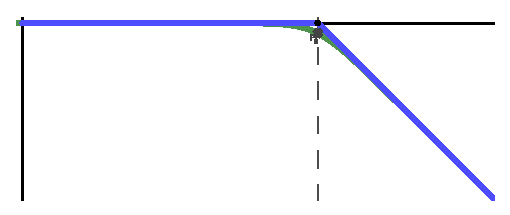
\includegraphics{RC_log_log_plot.eps}} % importing figure
\caption{Sketch of a log-log graph of attenuation against frequency} \label{fig:RC_log_log_plot}
\end{figure}
